\documentclass{article}
%\usepackage[austrian]{babel}

\input{epsf}

\usepackage{graphicx}

\usepackage[utf8]{inputenc}
\usepackage{amsmath}

% generic packages needed for math and logic symbols
\usepackage{amssymb}
\usepackage{stmaryrd}
\usepackage{mathrsfs}
\usepackage{array}

\usepackage{mathabx}

% for quotes
\usepackage{dirtytalk}
\newcommand{\saye}[1]{\emph{\say{#1}}}

%% for logical symbols 
%%% Logical operators
%% Common (but not filtered among those not needed)
\newcommand*{\lnextbase}{\ocircle}
\newcommand*{\lbackbase}{\circleddash}
\newcommand*{\lglobbase}{\square}
\newcommand*{\levenbase}{\Diamond}
\newcommand*{\luntilbase}{\mathbin{\mathcal{U}}}
\newcommand*{\lnextsup}[1]{\mathop{\lnextbase^{#1}}}
\newcommand*{\lbacksup}[1]{\mathop{\lbackbase^{#1}}}
\newcommand*{\lnextsub}[1]{\mathop{\lnextbase_{#1}}}
\newcommand*{\lbacksub}[1]{\mathop{\lbackbase_{#1}}}
\newcommand*{\lnextgen}[2]{\mathop{\lnextbase^{#1}_{#2}}}
\newcommand*{\lbackgen}[2]{\mathop{\lbackbase^{#1}_{#2}}}
\newcommand*{\lguntil}[4]{#3 \mathbin{\mathcal{U}^{#1}_{#2}} #4}
\newcommand*{\luntil}[3]{#2 \mathbin{\mathcal{U}^{#1}} #3}
\newcommand*{\lgsince}[4]{#3 \mathbin{\mathcal{S}^{#1}_{#2}} #4}
\newcommand*{\lsince}[3]{#2 \mathbin{\mathcal{S}^{#1}} #3}
\newcommand*{\lfuntil}[3]{#2 \mathbin{\mathcal{U}(#1)} #3}
\newcommand*{\lglob}[1]{\mathop{\lglobbase^{#1}}}
\newcommand*{\leven}[1]{\mathop{\levenbase^{#1}}}

%% LTL
\newcommand*{\lnext}{\mathop{\lnextbase}}
\newcommand*{\lluntil}[2]{#1 \mathbin{\mathcal{U}} #2}
\newcommand*{\llglob}{\mathop{\lglobbase}}
\newcommand*{\lleven}{\mathop{\levenbase}}

%% probability symbol
\newcommand*{\llprob}{\mathbb{P}}

%for the algorithm showing
\usepackage{algorithm}
\usepackage{algpseudocode}

% to add links to external resources
\usepackage{hyperref}
\hypersetup{
    colorlinks=true,
    linkcolor=blue,
    filecolor=magenta,      
    urlcolor=blue,    
    citecolor=black
}

%to list code in the document
\usepackage{listings}
\usepackage{xcolor}
\lstset{
  basicstyle=\ttfamily,
  columns=fullflexible,
}

%% bibliography management
\usepackage[backend=biber,style=numeric,sorting=ydnt]{biblatex}
\addbibresource{biblio.bib} %Import the bibliography file

%% to add todonotes
\usepackage{todonotes}

\newcommand\inParens[1]{\texttt{(}#1\texttt{)}}
\newcommand\inBraces[1]{\texttt{\{}#1\texttt{\}}}
\newcommand\comma{\texttt{,}}
\newcommand\semicolon{\texttt{;}}

\title{Model Checking ``MiniCheck''}

\setlength{\oddsidemargin}{0mm}
\setlength{\evensidemargin}{0mm}
\setlength{\topmargin}{-1cm}
\setlength{\textheight}{22.5cm}
\setlength{\textwidth}{15cm}

%\newcommand{\Nat}{\mbox{I\hspace{-0.1em}N}}
\newcommand{\Nat}{\ifmmode{\sf I\hspace*{-0.3mm}N} \else\mbox{${\sf I\hspace*{-0.3mm}N$}}\fi}
\newcommand{\nat}{\Nat}
\newcommand{\Reell}{\ifmmode{\sf I\hspace*{-0.3mm}R} \else\mbox{${\sf I\hspace*{-0.3mm}R$}}\fi}
\newcommand{\comment}[1]{}
\newcommand{\eqdef}{\mbox{$=_{df}\,$}}

\newcommand{\assnumber}{5}

\begin{document}
\large
\begin{center}
  {\Large \textbf{185.A05 Advanced Functional Programming SS 25}}  \\ [1ex] 
            Tuesday, 6 May 2025 \\
               {\Large \textbf{Assignment 4}} \\[.5ex]
              {\Large \textbf{Model Checking Project: MiniCheck}} \\[.5ex]
                 \textbf{All Chapters}  \\ [.75ex]
           \textbf{Topic:} Building a CTL Model Checker plus Implementing a Modelling extension \\[1ex]
          \textbf{Submission deadline:} Friday, 13th June 2025, noon (no continuous update)  \\ [0.5ex]
          \textbf{Contact:} prof. Jens Knoop, jens.knoop@tuwien.ac.at, \\
                            Francesco Pontiggia, francesco.pontiggia@tuwien.ac.at \\
                            Lou Elah Süsslin, lou.suesslin@student.tuwien.ac.at \\
                     (In case of need, this deadline will be extended (details posted via TUWEL))
\end{center}

\vspace{1ex}
\noindent
\noindent

\newcommand{\code}[1]{\texttt{#1}}

\noindent
The goal of the project is to implement a  Model Checker, \textit{MiniCheck}, 
for the so called Computational Tree Logic (CTL). 
The project consists of two parts: the core model checker and an extension. 

\paragraph{Part I - The MiniCheck Core.} The core model checker requires: 
\begin{itemize}
    \item a number of preliminary programming tasks dealing with Transition Systems (TS)
          and Computational Tree Logic (CTL) (cf.~Section \ref{subsec-ts} and \ref{subsec-ctl}).
    \item a verification module which checks an input CTL formula on a TS (cf.~Section \ref{subsec:mc}).
    \item a test suite allowing to validate the usability and correctness of the
          various components of the core (cf.~Section \ref{subsec-testsuite}).
\end{itemize}  
An illustrating example highlights the essence of model-checking in our setting (cf.~Section \ref{subsec:example}). 

\paragraph{Part II - The MiniCheck Extension.} The extension of the MiniCheck core concerns software model checking (cf.~Section \ref{sec:ext1}).

Note that the core is mandatory but is only worth a portion of the points achievable in this project. 
To achieve the full amount of points the extension has to be implemented, too.
However, it is not necessary for a positive grade. 
Additionally, there is a bonus task allowing to achieve even more than 
the full amount of points for the project (cf.~Section \ref{sec-bonus}). 
\bigskip

In Section \ref{sec:artefacts}, the submission artefacts are detailed. In contrast to previous assignments, you are not asked to implement functions with (often) given signatures. 
Instead, the functionality of the executed program is evaluated. 
You will have to design your own function signatures and data types and decide 
which data structures you want to use.

The program should not be written in a single file, but as a \href{https://docs.haskellstack.org/en/stable/README/}{\code{stack}} 
or \href{https://cabal.readthedocs.io/en/3.4/}{\code{cabal}} project consisting of multiple modules. 
It is encouraged to use custom and predefined data structures, as well as external libraries 
and Haskell language extensions \textbf{where appropriate}. It is not required to get the project to run on g0.

There will be a Q\&A session where help will be provided in case there are troubles with the selected technologies. 
The date will be announced via TUWEL news.

\section{Grading}
The preliminary programming tasks with two parsers at its core (cf.~Section \ref{subsec-ts} and \ref{subsec-ctl}), +
the verification module (cf.~Section \ref{subsec:mc}) and the test suite (cf.~Section \ref{subsec-testsuite}) 
of MiniCheck are mandatory. 
Implementing this core awards up to 300 points.
To gain more points on top of the aforementioned, you will have to implement the modelling
extension of the MiniCheck tool (see~Section \ref{sec:ext1}) 
or the bonus task (cf.~Section \ref{sec-bonus}). 
At most 400 points are awarded for the project implementation.
The project presentation (Demo) will be worth up to 200 points. 

The total points for the project are calculated by adding up the points on the core, 
the selected extensions and the presentation (for a maximum of 600 points).
For a positive evaluation of this project at least 300 points are required. 
A positive grade on the project is necessary in order to receive a positive grade in this course.
A positive grade on the core itself is \textit{not} required. 

In contrast to previous exercises, there is no possibility for a continuous update until the project demo.

\subsection{Note}
We do not assume an in-depth knowledge of model checking and its purpose, nor logics.
Some previous knowledge in related fields helps, but it's not mandatory,
as all used formalisms are introduced. 
This includes also:
\begin{itemize}
    \item Automata Theory
    \item Graph Algorithms
    \item Propositional Logics
\end{itemize}
See, e.g., \cite{BaKa} for deeper background details.

\section{MiniCheck Core (300 P)}

Model Checking consists of formally and exhaustively verifying a formula expressing some property
on all the possible executions of a particular type of automata (the \emph{model}). 
The model might be an abstract representation of a hardware component, or even a 
piece of software.
In the following, we provide some preliminary information 
about the type of the formalisms you are required to support, 
and then present the project to carry out. 

\subsection{Preliminaries - Transition Systems}
\label{subsec-ts}
As modelling formalism, we use \emph{Transition Systems} (TS). They are a particular variant 
of Finite State Automata which allow to describe adequately both hardware and software systems. 
Formally, a TS is a tuple ($S, Act, \rightarrow, I, AP, L$), where 
\begin{itemize}
    \item $S$ is a set of \emph{states},
    \item $Act$ is a set of \emph{actions},
    \item $\rightarrow\,\subseteq S \times Act \times S$ is a \emph{transition relation},
    \item $I \subseteq S$ is a set of \emph{initial states}.
    \item $AP$ is a set of \emph{atomic propositions}, and 
    \item $L : S \rightarrow 2^{AP}$ is a \emph{labelling function}.
\end{itemize}
The labelling function maps every state to the set of atomic propositions holding in that state. 
Informally, atomic propositions are just labels that carry information about states.
The initial state is chosen nondeterministically between all states $\in I$.
The transition system operates as follows: after having chosen an initial state $s \in I$, it chooses 
nondeterministically a transition $s \xrightarrow{\alpha} s'$, 
executes the action $\alpha$ and moves on to $s' \in S$. Note that a state may have outgoing transitions 
going to different states, but also 1) outgoing transitions to different states but associated with the same action, and
2) outgoing transitions to the same state but with different actions.
A \emph{run} of the TS is a valid \textbf{infinite} sequence of interleaved states and actions,
where valid just means that for each triple $s \alpha s'$ in the run the TS has a transition $s \xrightarrow{\alpha} s'$.

Note that, for simplicity sake, we consider only TS with no terminal states, i.e., 
every state has at least one outgoing edge. 
While this prevents some technical problems from occurring, 
it is not a limit to the expressive power of TS: for every state $s$ without outgoing edge, 
you can add a transition to a ``sink'' state $s_ {sink}$, 
and then define a self transition from $s_ {sink}$ to itself.

We adopt a \textbf{state-based} approach: we consider (and want to verify) 
the labels in the state sequence of a run of the TS, and abstract from actions, 
which are of no use in our verification algorithm. Then, in the following, we will consider
runs as sequence of states (\emph{paths}), and forget about actions.

\subsubsection*{Resources}
\cite[Paragraph 2.1]{BaKa}

\color{red}
\subsubsection*{Task 1}
Define:
\begin{itemize}
    \item a suitable plain-text representation of TS such that TS written in this representation
          can be passed as input to your tool, and
    \item a data type to represent them. 
    \item the type of the set of atomic propositions that can be used to label states of the Transition System. 
            Atomic Propositions (or atomic formulae) are boolean variables that represent either
            a description of the state (e.g., OFF and ON for a system that describes a lightbulb) 
            or a property that holds in the state (e.g. $nsoda == 0$ for a system that describes the functioning 
            of a soda vending machine, see the example in Section \ref{subsec:example}.).
\end{itemize} 
Implement: 
\begin{itemize}
    \item A parsing function from the plain-text representation of TS to the data type.
\end{itemize}
The parsing function should abort when it encounters a TS non complying with the syntax you defined.
Besides syntactic checks, we require you to implement some additional checks to detect 
non well-formed TS. Make sure that 1) there are no terminal states (or add the sink state),
2) there is at least an initial state,
and 3) that your formalisation of the set of atomic propositions is respected. 

\color{black}

You are allowed to choose one of the parsing approaches presented in the lecture or 
use an external monadic parsing library from Hackage. Document your choice.

We require that a state is always labelled with itself 
(i.e., $s_i \in L(s_i)$, which implies $S \subset AP$). 
This does not mean that the atomic propositions we consider are only state identifiers. 
As introduced earlier, a state may be labelled with different types of properties depending on the context: 
it will be up to you to define a suitable type to make your program be able to encode and 
deal with as many different situations as possible.

\subsection{Preliminaries - Computational Tree Logic (CTL)}
\label{subsec-ctl}

To express properties to verify on Transition Systems, we consider a temporal extension of propositional logic, 
i.e., the introduction of temporal modalities on top of propositional logic, to reason about the temporal ordering
of events.

In particular, the temporal modalities we consider are $\ovoid$ (pronounced ``next'') 
and $\luntilbase$ (pronounced ``until''). These temporal modalities allow to constrain the future states 
that can be visited in a run from an initial state. They are operators part of the so called Computation Tree Logic (CTL).
Note here the difference between temporal ordering and timing: in temporal logics time is seen as a discrete sequence of time instances 
(or snapshots, if you like), and not as a continuous variable. With these formalism, 
you do not specify something like ``A for two seconds, then B for one second", but rather ``A, and in the next time instance B".

In particular, CTL (differently with respect to some other logics, e.g. LTL) is based on a \emph{branching} notion of time. 
Branching time refers to the fact that every step in a path of the TS is associated with a choice between 
different successor states, which is a split between several different futures. 
All the possible paths that arise from a state can then be represented
as a tree of states of infinite depth, where each choice of a successor in a state is between all the subtrees generated by all the successor states.
By fixing a successor for every state in the tree, we get one of all possible futures, 
i.e., a single path, a traversal of the TS.

Computation Tree Logic (CTL) thus allows to express properties that must hold for \emph{some} or \emph{all} paths starting in a state. 
For this purpose, it features two operators: an existential path quantifier ($\exists$) and a universal path quantifier ($\forall$). 
Intuitively, $\exists \varphi$ holds in a state if there exists \emph{some} path starting in that state satisfying $\varphi$. 
Dually, $\forall \varphi$ holds in a state if \emph{all} paths starting in that state satisfy $\varphi$.

\subsubsection*{CTL Syntax}
Given a set $AP$ of atomic propositions, with $a \in AP$, CTL formulae follow the following syntax: 
\begin{align*}
    \emph{state formula } & \Phi ::= \text{true} \mid a \mid \Phi_1 \land \Phi_2 \mid \neg \Phi \mid \exists \, \varphi \mid \forall \, \varphi \\
    \emph{path formula }  & \varphi ::= \lnext{\Phi} \mid \lluntil{\Phi_1}{\Phi_2} \\
\end{align*}
Greek capital letters denote CTL state formulae, whereas lowercase Greek letters denote CTL path formulae. 
A well defined CTL formula is a CTL state formula.

\subsubsection*{CTL Semantics}
Given atomic proposition $a \in AP$, $TS = (S, Act, \rightarrow, I, AP, L)$, state $s \in S$, 
CTL state formulae $\Phi, \Psi$, CTL path formula $\varphi$, 
the semantics of CTL is defined in terms of the following satisfaction relation $\vDash$ (read ``satisfies").

For state $s$ and CTL (state) formula $\varphi$, $s \vDash \Phi$ if and only if $\Phi$ holds in $s$.
\begin{alignat*}{3}
     & s \vDash \text{true} &  \\
     & s \vDash a & \text{ iff } & a \in L(s) \text{ i.e., $a$ is a label of $s$}\\ 
     & s \vDash \neg \Phi & \text{ iff } & \text{not } s \vDash \Phi \\
     & s \vDash \Phi \land \Psi \, \, & \text{ iff }&  s \vDash \Phi \text{ and } s \vDash \Psi \\
     & s \vDash \exists \, \varphi & \text{ iff } & \pi \vDash \varphi \text{ for some } \pi \in Paths(s) \\ 
     & s \vDash \forall \, \varphi & \text{ iff } & \pi \vDash \varphi \text{ for all } \pi \in Paths(s) \\ 
\end{alignat*}

Given a path $\pi$ (a sequence of states), $\vDash$ is defined for path formulae as follows: 
\begin{alignat*}{3}
    & \pi \vDash \lnext{\Phi} & \text{ iff     } & \pi[1]  \vDash \Phi \\ 
    & \pi \vDash \lluntil{\Phi}{\Psi} \, \, & \text{ iff    } & \exists j \geqslant 0 \, . \, (\pi[j]  \vDash \Psi \land (\forall 0 \leqslant k < j \, . \,  \pi[k]  \vDash \Phi))
\end{alignat*}

A TS satisfies CTL formula $\Phi$ if and only if all initial states of the TS satisfy $\Phi$.

\subsubsection{Derived Operators}

In addition, we introduce the following well-known \emph{derived} Boolean operators from propositional logic for state formulae.
\begin{align*}
    &\; \Phi_1 \lor \Phi_2 \equiv \neg (\neg \Phi_1 \land \neg \Phi_2) \\
    &\; \Phi_1 \rightarrow \Phi_2 \equiv \neg \Phi_1 \lor \Phi_2 \\
    &\; \Phi_1 \leftrightarrow  \Phi_2 \equiv (\Phi_1 \rightarrow \Phi_2) \land (\Phi_2 \rightarrow \Phi_1) \\
    &\; \Phi_1 \oplus  \Phi_2 \equiv (\Phi_1 \land \neg \Phi_2) \lor (\Phi_2 \land \neg \Phi_1)\\
\end{align*}

We derive also some more temporal modalities for path formulae: 
\begin{itemize}
    \item $\lleven$ (pronounced ``eventually''), and
    \item $\llglob$ (pronounced``generally/always");
\end{itemize}
Intuitively, $\lleven$ means \saye{at some point in the path}, and $\llglob$ means \saye{always in the path}.

These operators can be derived from the base operators through the following
\begin{align*}
    &\; \exists \lleven \Phi \equiv \exists(\lluntil{\text{true}}{\Phi}) \\ 
    &\; \forall \lleven \Phi \equiv \forall(\lluntil{\text{true}}{\Phi}) \\ 
    &\; \\ 
    &\; \exists \llglob \Phi \equiv \neg\forall \lleven \neg\Phi \\ 
    &\; \forall \llglob \Phi \equiv \neg\exists \lleven \neg\Phi \\
\end{align*}
We give an informal notion of some of these formulae. The left hand side of the first equivalence means \saye{there exists a path such that at some point $\Phi$ holds}.
The right hand side of the second equivalence means \saye{on all paths, anything holds until $\Phi$ holds}.

You are required to handle also derived operators.

\subsubsection*{Hint about derived operators}
If your code translates formulae with derived operators into formulae 
with only base operators through these equivalence rules, you will have implemented support of 
derived operators for free (even if performances will suffer).

\color{red}
\subsubsection*{Task 2}
Define:
\begin{itemize}
    \item a suitable plain-text representation of CTL formulae such that formulae written in this representation can be passed as input to your tool, and 
    \item a data type to represent them.
    \item the type of the set of atomic propositions (APs) that can be used in the formulae. Note that they should 
            match the APs of the transition system.
\end{itemize}
\color{black}

\subsubsection*{Note}
It is up to you to decide how to combine the two plain text representations of the inputs (the TS and the formula) 
(e.g., both in the same file, in two separate files \dots), 
and how to provide them to the Model Checker via some command-line arguments 
(e.g., the folder path, two paths, \dots). 
Any potential issue with command line arguments must be treated adequately 
(e.g., missing arguments, too many arguments, wrong arguments, \dots).

The results of a model check query should be printed on the CLI (command line interface), 
together with some additional information/logging you may find useful.
(e.g. ``Parsing formula from file \dots")

\subsubsection*{Resources}
For a complete definition of CTL, \cite[Paragraph 6.2 (in particular 6.1.1 and 6.1.2)]{BaKa}.

\subsection{The Model Checking procedure}
\label{subsec:mc}
Given a TS $\mathcal{A}$ and a CTL formula $\Phi$ we want to verify whether $\mathcal{A} \vDash \Phi$.
In order to do so, we have to establish whether $\Phi$ is satisfied in each initial state $s$ of $\mathcal{A}$.
The model checking procedure is roughly composed of two steps: 
\begin{itemize}
    \item computing the set $Sat(\Phi)$ of all states of $\mathcal{A}$ satisfying $\Phi$ (recursively), and
    \item checking whether all initial states $s \in I$ belong to $Sat(\Phi)$; 
\end{itemize}
In other words, $\mathcal{A} \vDash \Phi$ if and only if $I_{\mathcal{A}} \subseteq Sat(\Phi)$.
The model checking procedure is essentially a bottom-up traversal of the parse tree of $\Phi$ - we compute
for each subformula its satisfaction set, and then compose them bottom up to compute $Sat(\Phi)$.

\subsubsection{Remark about the notation}
In the following, we present a procedure which computes the satisfaction sets for formulae of 
CTL expressed in the so called \emph{existential normal form} (ENF). The set of formulae in ENF is given by: 
\begin{align*}
    & \Phi ::= \text{true} \mid a \mid \Phi_1 \land \Phi_2 \mid \neg \Phi \mid \exists \lnext{\Phi} \mid \exists (\lluntil{\Phi_1}{\Phi_2}) \mid \exists \llglob \Phi \\
\end{align*}
We see that the $\forall$ operator is not present in CTL formulae in ENF.
Again, you can either define by yourself the satisfaction set for all CTL formulae, 
or, you can translate the remaining formulae in EFN (which is the easier way).
The translation rules are (\cite[Paragraph 6.2.4]{BaKa}):
\begin{alignat*}{2}
    & \forall \lnext{\Phi} & \equiv \,\, & \neg \exists \lnext{\neg \Phi} \\
    & \forall \big( \lluntil{\Phi}{\Psi} \big) \, & \equiv \, \, & \neg \exists \big( \lluntil{\neg \Psi}{(\neg \Phi \land \neg \Psi)} \big) \land \neg \exists \llglob \neg \Psi \\
\end{alignat*}

\subsubsection{The algorithm}
The following algorithm sketches the procedure. 

\begin{algorithm}[H]
    \caption{CTL Model Checking}
    \hspace*{\algorithmicindent} \emph{Input}: finite transition system $\mathcal{A}$ and CTL formula $\Phi$ (both over $AP$) \\
    \hspace*{\algorithmicindent} \emph{Output}: ``yes'' if $TS \vDash \Phi$; otherwise, ``no''
    \begin{algorithmic}[1]
    \Function{$SatFun$}{$\phi$}
        \If{$\phi$ contains state subformulae}
            \State // for children nodes $\psi_1, \psi_2$ of the parse tree of $\phi$
            \State $Sat(\psi_1) = SatFun(\psi_1)$; $Sat(\psi_2) = SatFun(\psi_2)$ 
            \State combine $Sat(\psi_1), Sat(\psi_2)$ depending on the operator of $\phi$ ($\land, \exists\lnext, \exists \, \mathbin{\mathcal{U}}, \exists\llglob$)
            \State // see the characterization below
        \Else
            \State compute directly the set $Sat(\phi)$.
        \EndIf
        \State return $Sat(\phi)$.
    \EndFunction
    \State
    \State $SatSet$ := $SatFun(\Phi)$
    \State \textbf{return $I_{\mathcal{A}} \subseteq SatSet$.}
    \end{algorithmic}
\end{algorithm}

\subsubsection*{Characterization of $Sat(\cdot)$ for CTL formulae in ENF}
We now formally define the set $Sat(\cdot)$ for every formula.
Let TS $ = (S, Act, \rightarrow, I, AP, L)$ be a transition system without terminal states. 
For all CTL formulae $\Phi$, $\Psi$ over $AP$ it holds:
\begin{alignat*}{3}
    & Sat(\text{true})          && := S \\
    & Sat(a)                    && := \{ s \in S \mid a \in L(s) \}, \text{ for any a } \in AP \\ 
    & Sat( \Phi \land \Psi)     && := Sat(\Phi) \cap Sat(\Psi) \\ 
    & Sat(\neg \Phi)            && := S \, \setminus \, Sat(\Phi) \\ 
    & Sat(\exists \lnext{\Phi}) && := \{ s \in S \mid Post(s) \cap Sat(\Phi) \neq \varnothing \}\\
    & Sat\big(\exists (\lluntil{\Phi}{\Psi}) \big) && \text{ is the smallest subset T of S such that:} \\
    &&& \text{ (1) } Sat(\Psi) \subseteq T \text{ and } \\
    &&& \text{ (2) } s \in Sat(\Phi) \text{ and } Post(s) \cap T \neq \varnothing \text{ implies } s \in T \\
    & Sat(\exists \llglob \Phi) && \text{is the largest subset T of S such that:}\\
    &&& \text{ (3) } T \subseteq Sat(\Phi) \text{ and } \\
    &&& \text{ (4) } s \in T \text{ implies } Post(s) \cap T \neq \varnothing \\
\end{alignat*}
where
\begin{align*}
    Post(s) := \bigcup_{\alpha \in Act} \{ s' \in S \mid s \xrightarrow{\alpha} s' \}
\end{align*}
is just the set of successors of a state.

\subsubsection{How to compute $Sat(\cdot)$}
For most cases, you can just stick to the definition. There are only two critical situations.
To compute $Sat\big(\exists \, (\lluntil{\Phi}{\Psi}) \big)$ and $Sat(\exists \llglob \Phi)$, 
an iterative approach is required to compute respectively the smallest subset and the greatest subset 
that satisfy the respective conditions. The two algorithms are sketched here.

\begin{algorithm}[H]
    \caption{Computation of the satisfaction set for Until formulae}
    \hspace*{\algorithmicindent} \emph{Input}: finite transition system TS with state set S and CTL formula $\Phi_1 := \exists (\lluntil{\Phi}{\Psi})$.\\
    \hspace*{\algorithmicindent} \emph{Output}: $Sat(\Phi_1) = \{ s \in S \mid s \vDash \Phi_1 \}$.
    \begin{algorithmic}[1]
        \State T := $Sat(\Psi)$; (* compute the smallest fixpoint *)
        \While { $\{ s \in Sat(\Phi) \, \setminus \, T \mid Post(s) \cap T \neq \varnothing \} \neq \varnothing $}
            \State $ T := T \cup \{ s \in Sat(\Phi) \, \setminus \, T \mid Post(s) \cap T \neq \varnothing \} $;
        \EndWhile
    \State \textbf{return} T;
    \end{algorithmic}
\end{algorithm}

Intuitively speaking, at iteration $i$ of the while loop, the set $T_i$ contains all states
that can reach a $\Psi$-state in at most $i$ steps via a path passing only through $\Phi$ states.

\begin{algorithm}[H]
    \caption{Computation of the satisfaction set for Existential Always formulae}
    \hspace*{\algorithmicindent} \emph{Input}: finite transition system TS with state set S and CTL formula $\Phi_1 := \exists (\llglob \Phi)$. \\
    \hspace*{\algorithmicindent} \emph{Output}: $Sat(\Phi_1) = \{ s \in S \mid s \vDash \Phi_1 \}$.
    \begin{algorithmic}[1]
        \State T := $Sat(\Phi)$; (* compute the greatest fixpoint *)
        \While { $\{ s \in T \mid Post(s) \cap T = \varnothing \} \neq \varnothing$ }
            \State $ T := T \, \setminus \, \{ s \in T \mid Post(s) \cap T = \varnothing \} $;
        \EndWhile
    \State \textbf{return} T;
    \end{algorithmic}
\end{algorithm}

\subsubsection{Detailed Algorithms for Until and Existential Always formulae}
The following algorithm is a potential implementation in a ``backward'' manner
of the computation of $Sat(\cdot)$ for Until formulae, 
assuming your representation of the Transition System allows to 
quickly access the predecessors of a state, defined as 
\begin{align*}
    Pre(s) := \bigcup_{\alpha \in Act} \{ s' \in S \mid s' \xrightarrow{\alpha} s \}
\end{align*}
The basic idea is to compute $Sat\big(\exists \, (\lluntil{\Phi}{\Psi}) \big)$ by means of the iteration: 
\begin{alignat*}{3}
    T_0 = Sat(\Psi) & \text{ and } & T_{i+1} = T_i \cup \{ s \in Sat(\Phi) \mid Post(s) \cup T_i \neq \varnothing \} \\
\end{alignat*}
until a fixpoint is reached, i.e. until $T_i = T_{i+1}$.

\begin{algorithm}[H]
    \caption{Enumerative backward search for computing $Sat\big(\exists \, (\lluntil{\Phi}{\Psi}) \big)$}
    \hspace*{\algorithmicindent} \emph{Input}: finite transition system TS with state set S and CTL formula $\Phi_1 := \exists (\lluntil{\Phi}{\Psi})$ \\
    \hspace*{\algorithmicindent} \emph{Output}: $Sat(\Phi_1) = \{ s \in S \mid s \vDash \Phi_1 \}$
    \begin{algorithmic}[1]
        \State $E := Sat(\Psi)$;
        \State $T := E$;
        \While { $ E \neq \varnothing $}
            \State \textbf{let} $s' \in E$;
            \State $E := E \setminus \{ s' \}$;
            \For{$s \in Pre(s')$}
                \If{$s \in Sat(\Phi) \setminus T$}
                    \State $E := E \cup \{s\}$;
                    \State $T := T \cup \{s\}$;
                \EndIf
            \EndFor
        \EndWhile
    \State \textbf{return} T;
    \end{algorithmic}
\end{algorithm}

Likewise, the following algorithm is a potential implementation in a ``backward'' manner 
of the computation of $Sat(\cdot)$ for Existential Always formulae. The basic idea is to 
compute $Sat(\exists \, \llglob \Phi)$ by means of the iteration: 
\begin{alignat*}{3}
    T_0 = Sat(\Phi) & \text{ and } & T_{i+1} = T_i \cap \{ s \in Sat(\Phi) \mid Post(s) \cup T_i \neq \varnothing \} \\
\end{alignat*}
until a fixpoint is reached. The algorithm makes use of an additional counter vector $count$.

\begin{algorithm}[H]
    \caption{Enumerative backward search for computing $Sat(\exists \llglob \Phi)$}
    \hspace*{\algorithmicindent} \emph{Input}: finite transition system TS with state set S and CTL formula $\Phi_1 := \exists \llglob \Phi$ \\
    \hspace*{\algorithmicindent} \emph{Output}: $Sat(\Phi_1) = \{ s \in S \mid s \vDash \Phi_1 \}$
    \begin{algorithmic}[1]
        \State $E := S \, \setminus \, Sat(\Phi)$;
        \State $T := Sat(\Phi)$;
        \For{$s \in Sat(\Phi)$}
            \State $count[s] := \, \, | Post(s) | $; 
        \EndFor 
        \While { $ E \neq \varnothing $}
            \State \textbf{let} $s' \in E$;
            \State $E := E \, \setminus \, \{ s' \}$;
            \For{$s \in Pre(s')$}
                \If{$s \in  T$}
                    \State $count[s] := count[s] -1$;
                    \If{$count[s] == 0$}
                        \State $T := T \, \setminus \, \{s\}$;
                        \State $E := E \cup \{s\}$;
                    \EndIf 
                \EndIf
            \EndFor
        \EndWhile
    \State \textbf{return} T;
    \end{algorithmic}
\end{algorithm}



\subsubsection{Resources}
\cite[Paragraph 6.4]{BaKa}

\color{red}
\subsubsection*{Task 3}
\begin{itemize}
    \item Define a suitable data type reperesentation of CTL formulae in Existential Normal Form.
    \item Implement a function converting CTL formulae not in ENF into ones in ENF.
    \item Implement the CTL model checking Algorithm 1 presented here by using, if you like, Algorithms 4 and 5.
\end{itemize}

\color{black}

\subsection{Test Suite}
\label{subsec-testsuite}
Projects of this size profit from an automatic test-suite. 
Write a test-suite for the major components of the project using one of the following frameworks:

\begin{itemize}
\item \href{https://hackage.haskell.org/package/hspec}{\texttt{hspec}}, a tutorial can be found \href{https://hspec.github.io/}{\texttt{here}}
\item \href{https://hackage.haskell.org/package/tasty}{\texttt{tasty}}
\item \href{https://hackage.haskell.org/package/HTF}{\texttt{HTF}}
\item \href{https://hackage.haskell.org/package/HUnit}{\texttt{HUnit}}
\end{itemize}

As before, it is encouraged to utilise external libraries for writing tests.

It is required to write at least three unit tests for the components of
Section \ref{subsec-ts} and \ref{subsec-ctl}, and a test unit for the
components of Section \ref{subsec:mc}.

\subsection{Example} \label{subsec:example}
We give now an example of a Transition System and some formulae that hold for it. The example has been taken from \cite[Paragraph 2.1]{BaKa}.
The following picture represents a preliminary design of a beverage vending machine. 
The machine can either deliver beer or soda. States are indicated by ovals and transitions by labelled edges. 
Every state is labelled with some description of the state itself. Initial states are indicated by having an incoming arrow without source.
\begin{figure}[H]
  \begin{center}
      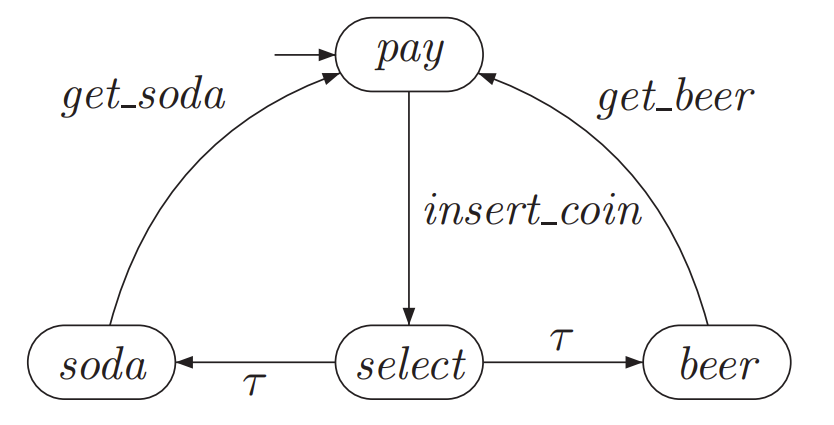
\includegraphics[scale = 0.50]{pictures/example.png}
  \end{center}
\end{figure}
The following formulae hold for this TS - note, $\tau$ denotes an internal transition:
\begin{alignat*}{3}
    \forall \lleven \text{pay} \, \, \, &  \text{:= \saye{every path will eventually return to the ``pay'' state.}} \\
    \exists \lleven \text{soda} \, \, \, & \text{:= \saye{there is a path which eventually reaches the granting of a soda.}} \\
    \exists \lleven \text{soda} \, \, \, & \text{:= \saye{there is a path which eventually reaches the granting of a soda.}} \\
    \forall \llglob (\text{select} \implies (\forall \lnext \neg \text{select})) \, \, \, & \text{:= \saye{on every path, a ``select'' cannot be followed by another ``select''.}} \\
\end{alignat*}
The following formula does not hold for the TS:
\begin{alignat*}{3}
    \forall (\lleven \text{ soda}) \, \, \, & \text{:= \saye{every path with eventually reach the granting of a soda.}} \\ 
\end{alignat*}
This is not true, because the path which always selects the beer is feasible, and violates the specification.
Also
\begin{alignat*}{3}
    \hspace*{-5em}\exists \llglob \big(\text{ select } \implies  (\forall \lnext \text{ soda })\big) & \text{:= \saye{there is a path where all ``select'' states can be followed by ``soda'' states only.}} \\ 
\end{alignat*}
is not true, because the only ``select'' state in the model can be followed by both a ``soda'' and 
a ``beer'' state.
\clearpage
\section{Extension - Parsing MINI$^{--}$ Programs (100 P)}
\label{sec:ext1}
With this extension, you are required to extend the modelling power of MiniCheck targeting 
software verification. While TS are good for expressing hardware models, they may be too low-level 
to model software programs. To help the user of your version of MiniCheck, we will implement an 
automated translation procedure for programs written in a toy programming language, MINI$^{--}$, into TS.

\subsection{Informal Description}
This section informally describes the core of the MINI$^{--}$ programming language, 
only covering the language core.

MINI$^{--}$ is a procedural programming language. 
The syntax and semantics of MINI$^{--}$ are inspired by the \href{https://en.wikipedia.org/wiki/C_(programming_language)}{programming language C}.

All code is contained in a single procedure \code{main} and variables are of the same type, 
namely the boolean type. This means that the type of the variables is not explicitly specified in MINI$^{--}$. 
Variables are not required to be declared before definition.
However, it is necessary to define their value before usage, 
i.e.~a variable must be initialised before it can be used in boolean expressions.

The procedure \code{main} implements an impure function, 
where input/output functionality \textbf{is  included in the core of MINI$^{--}$}. 
Procedure \code{main} takes a defined set of named variables and returns a result. 
Regarding the variables in the argument lists, 
you need to consider all possible combinations of assignments of values for them.

The last statement of the procedure must be a \code{return} statement and no other \code{return} statement can occur in the procedure. 
The \code{if} statement is defined as in C. It executes either the first or optionally the second block.

Modern programming languages usually have a way to interact with a user via terminal or file system. 
We consider two statements: one that prints a boolean and one that reads a boolean value.
While these statements are a major issue for the interpreter, 
and it's hard to define their semantics in terms of a pure evaluation function, 
in the model checking problem they can be treated just as a source of non-determinism, 
which is already there in the type of Transition Systems we are using.

\subsection{Syntax}

\begin{align*}
program :=& \ \texttt{procedure main}\inParens{argument\_vars} \inBraces{procedure\_body} \\
argument\_vars :=& \ var \ | \ var\comma argument\_vars \\
procedure\_body :=& \ statements \quad return\_stmt \\ \\
statements :=& \ \varepsilon \ | \ statement \quad statements \\
statement :=&  \ if\_stmt \ | \ assign\_stmt \ | \ print\_bool\_stmt \ | \ read\_bool\_stmt\\
if\_stmt :=& \ \texttt{if}\inParens{bool\_expr} \inBraces{statements}\\
& \ | \ \texttt{if}\inParens{bool\_expr} \inBraces{statements} \texttt{else}\inBraces{statements} \\
assign\_stmt :=& \ var \texttt{=} bool\_expr \semicolon \\
print\_bool\_stmt :=& \ \texttt{print\_bool}\inParens{bool\_expr}\semicolon \\
read\_bool\_stmt :=& \ var \texttt{=}\texttt{read\_bool}\inParens{}\semicolon \\
bool\_expr :=& \ bool\_expr\_nested \ | \ \neg bool\_exp\_nested \\
& \ | \ bool\_expr\_nested \quad relator \quad bool\_expr\_nested \\
bool\_expr\_nested :=& \ bool \ | \ var \ | \ (bool\_expr) \\
relator :=& \ \land \ | \ \lor \ | \ \implies \ | \ \iff | \ \oplus \\
return\_stmt :=& \ \texttt{return }\space bool\_expr \semicolon\\
bool :=& \ \texttt{true} \ | \ \texttt{false} \\
var :=& \ ident \\
ident :=& \ char \quad ident\_rest \\
ident\_rest :=& \ \varepsilon \ | \ ident\_char \quad ident\_rest \\
ident\_char :=& \ char \ | \ digit \ | \ \texttt{\_} \\
char :=& \ \texttt{a} \ | \ \ldots \ | \ \texttt{z} \\
digit :=& \ \texttt{0} \ | \ \ldots \ | \ \texttt{9}
\end{align*}

Additional whitespace is allowed everywhere except within identifier names, integer literals, 
the binary comparison operators, and the keywords (\code{procedure}, \code{return}, \code{if}, \code{else}, \code{while}).

\subsection{Semantics}
We define now the semantics of a MINI$^{--}$ program $\texttt{P}$ in terms of a Transition System, 
through the so-called \textbf{structural operational semantics (SOS)}. 
With this semantics, we mimic the step-by-step execution of the program 
through the transition relation of a Transition System. 
We follow the inference rules of the SOS to construct 
the state set and the transition relation of the corresponding TS.

A state of the TS corresponds to the current program counter (i.e., the next instruction to be executed), 
and the current valuation of all the already occurred program variables $\gamma$.
Formally, a state is given by $\langle \texttt{P}, \mathbf{\gamma} \rangle$, where program $\texttt{P}$ is just 
viewed as a sequence of statements.

\subsubsection{The set of initial states}
The set of initial state of a Transition System $I$ is composed by all possible combinations 
of initial boolean values for the set of arguments of the MINI$^{--}$ program $\texttt{P}$. 
This can be represented in set notation by $2^{arg(\texttt{P})}$, where $arg$ is the set of arguments of $\texttt{P}$. 
A subset of $arg$ contains all and only the variables that are evaluated to true in the current evaluation. 
The set of initial states is then defined as:
\begin{align*}
    I := \{ \langle \texttt{P}, \mathbf{\gamma} \rangle \mid \mathbf{\gamma} \in 2^{arg(\texttt{P})} \}
\end{align*}

\subsubsection{The Transition Relation}
The transition relation is then defined by the following transition rules, 
where the symbol $\downarrow$ indicates a state where there is no more statement to evaluate.
\begin{align*}
    &\; \frac{\varphi \notin \gamma}{\langle \texttt{ if}(\varphi)\texttt{\{B\};P}, \, \,  \mathbf{\gamma} \rangle \rightarrow \lightning} &&\;
      \frac{\varphi \notin \gamma}{\langle \texttt{ if}(\varphi)\texttt{\{B\}else\{E\};P}, \, \, \mathbf{\gamma} \rangle \rightarrow \lightning} \\ \\
    &\; \frac{\mathbf{\gamma} \vDash \varphi}{\langle \texttt{ if}(\varphi)\texttt{\{B\};P}, \, \,  \mathbf{\gamma} \rangle \rightarrow \langle \texttt{ B;P}, \, \,  \mathbf{\gamma} \rangle} &&\;
      \frac{\mathbf{\gamma} \nvDash \varphi}{\langle \texttt{ if}(\varphi)\texttt{\{B\};P}, \, \, \mathbf{\gamma} \rangle \rightarrow \langle \texttt{P}, \, \, \mathbf{\gamma} \rangle} \\ \\
    &\; \frac{\mathbf{\gamma} \vDash \varphi}{\langle \texttt{ if}(\varphi)\texttt{\{B\}else\{E\};P}, \, \, \mathbf{\gamma} \rangle \rightarrow \langle \texttt{ B;P}, \, \, \mathbf{\gamma} \rangle} &&\;
      \frac{\mathbf{\gamma} \nvDash \varphi}{\langle \texttt{ if}(\varphi)\texttt{\{B\}else\{E\};P}, \, \, \mathbf{\gamma} \rangle \rightarrow \langle \texttt{ E;P}, \, \, \mathbf{\gamma} \rangle} \\ \\
    &\;\frac{\mathbf{\gamma} \vDash (bool\_expr \mapsto v)}{\langle var\texttt{=}bool\_expr\texttt{;P}, \, \, \mathbf{\gamma} \rangle \rightarrow \langle \texttt{P}, \, \, \mathbf{\gamma}[var \mapsto v] \rangle } &&\;
      \frac{bool\_expr \notin \gamma}{\langle var\texttt{=}bool\_expr\texttt{;P}, \, \, \mathbf{\gamma} \rangle \rightarrow \lightning } \\  \\
    &\;\frac{bool\_expr \in \gamma}{\langle \texttt{print\_bool(}bool\_expr\texttt{);P}, \, \,  \mathbf{\gamma}\rangle \rightarrow \langle \texttt{P}, \mathbf{\gamma} \rangle} &&\;
       \frac{bool\_expr \notin \gamma}{\langle \texttt{print\_bool(}bool\_expr\texttt{);P},  \, \, \mathbf{\gamma}\rangle \rightarrow \lightning} \\  \\
    %&\;\frac{x \notin \gamma}{\langle x=read\_bool;P , \mathbf{\gamma} \rangle \rightarrow \lightning} &&\; \\ \\
    &\;\frac{var \in \gamma}{\langle var\texttt{=read\_bool();P}, \, \, \mathbf{\gamma} \rangle \rightarrow \langle \texttt{P}, \, \, \mathbf{\gamma}[var \mapsto T] \rangle} &&\;
       \frac{var \in \gamma}{\langle var\texttt{=read\_bool();P}, \, \, \mathbf{\gamma} \rangle \rightarrow \langle \texttt{P}, \, \, \mathbf{\gamma}[var \mapsto F] \rangle }\\ \\
    &\;\frac{bool\_expr \in \gamma}{\langle \texttt{return } bool\_expr\texttt{;}, \, \, \mathbf{\gamma} \rangle \rightarrow \langle \downarrow, \, \, \mathbf{\gamma} \rangle} &&\;
       \frac{bool\_expr \notin \gamma}{\langle \texttt{return } bool\_expr\texttt{;}, \, \, \mathbf{\gamma} \rangle \rightarrow \lightning} \\ \\
    &\;\frac{}{\langle \downarrow, \mathbf{\gamma} \rangle \rightarrow \langle \downarrow, \mathbf{\gamma} \rangle} &&\;
       \frac{}{\langle \lightning, \mathbf{\gamma} \rangle \rightarrow \langle \lightning, \mathbf{\gamma} \rangle} \\
\end{align*}

We use the notation $\mathbf{\gamma}[var \mapsto v]$ to denote the state that is obtained 
when updating the value of the variable $var$ to $v$. 

A statement is invalid if it uses a variable $var$ that has not been defined before.
We use notation $var \notin \gamma$ to indicate that variable $var$ has no binding in 
the current state. With a slight abuse of notation, we use $bool\_expr \notin \gamma$ or $\varphi \notin \gamma$
to indicate that a variable with no binding occurs in $bool\_expr$ or $\varphi$. An invalid statement makes the
whole program invalid. This is represented in our semantics with a transition 
to an error state indicated with $\lightning$.

\subsubsection*{Note about terminal states}
The last two rules have been added due to a technical problem. 
While MINI$^{--}$ programs are guaranteed to terminate for any input or to reach the error state, 
the Transition Systems we have considered don't have terminal states, i.e.~that every state has at least one outgoing edge. 
To accommodate the two formalisms, we introduce a self loop in the final states of the program, 
which induces the required infinite runs in the Transition System.

\subsubsection*{Note about model checking}
When verifying properties like \saye{Variable \texttt{x} must be false after one step for all paths}, 
we encounter the problem that variable $\texttt{x}$ may not be initialized after one step
(i.e., $\texttt{x} \notin \gamma$ at that point of the execution). 
In such cases, MiniCheck assumes $\texttt{x}$ to be false. In other words, 
a variable is considered by the model checking procedure to be false until it is set to be true.
There is not need to distinguish in model checking between an unitialized variable and a false one.
You need however to do it in the semantics of MINI$^{--}$, where it makes a difference.

\clearpage
\subsection{Example}
A procedure over two inputs:
\begin{lstlisting}[escapeinside={(*}{*)}]
procedure main(a, b) {
    if (a) { c = (* $\neg$ *)(b); 
    } else { c = b; }
    d = c (* $\oplus$ *) true;
    return d;
}
\end{lstlisting}
The corresponding Transition System, where initial states are at the top. 
An example formula on this program is $\exists \lleven (return \land d)$,
which simply means \saye{there is a path returning value 1}. This formula holds for this TS 
because of the leftmost path. Also $\forall \lleven return$ holds.
\begin{figure}[H]
    \begin{center}
        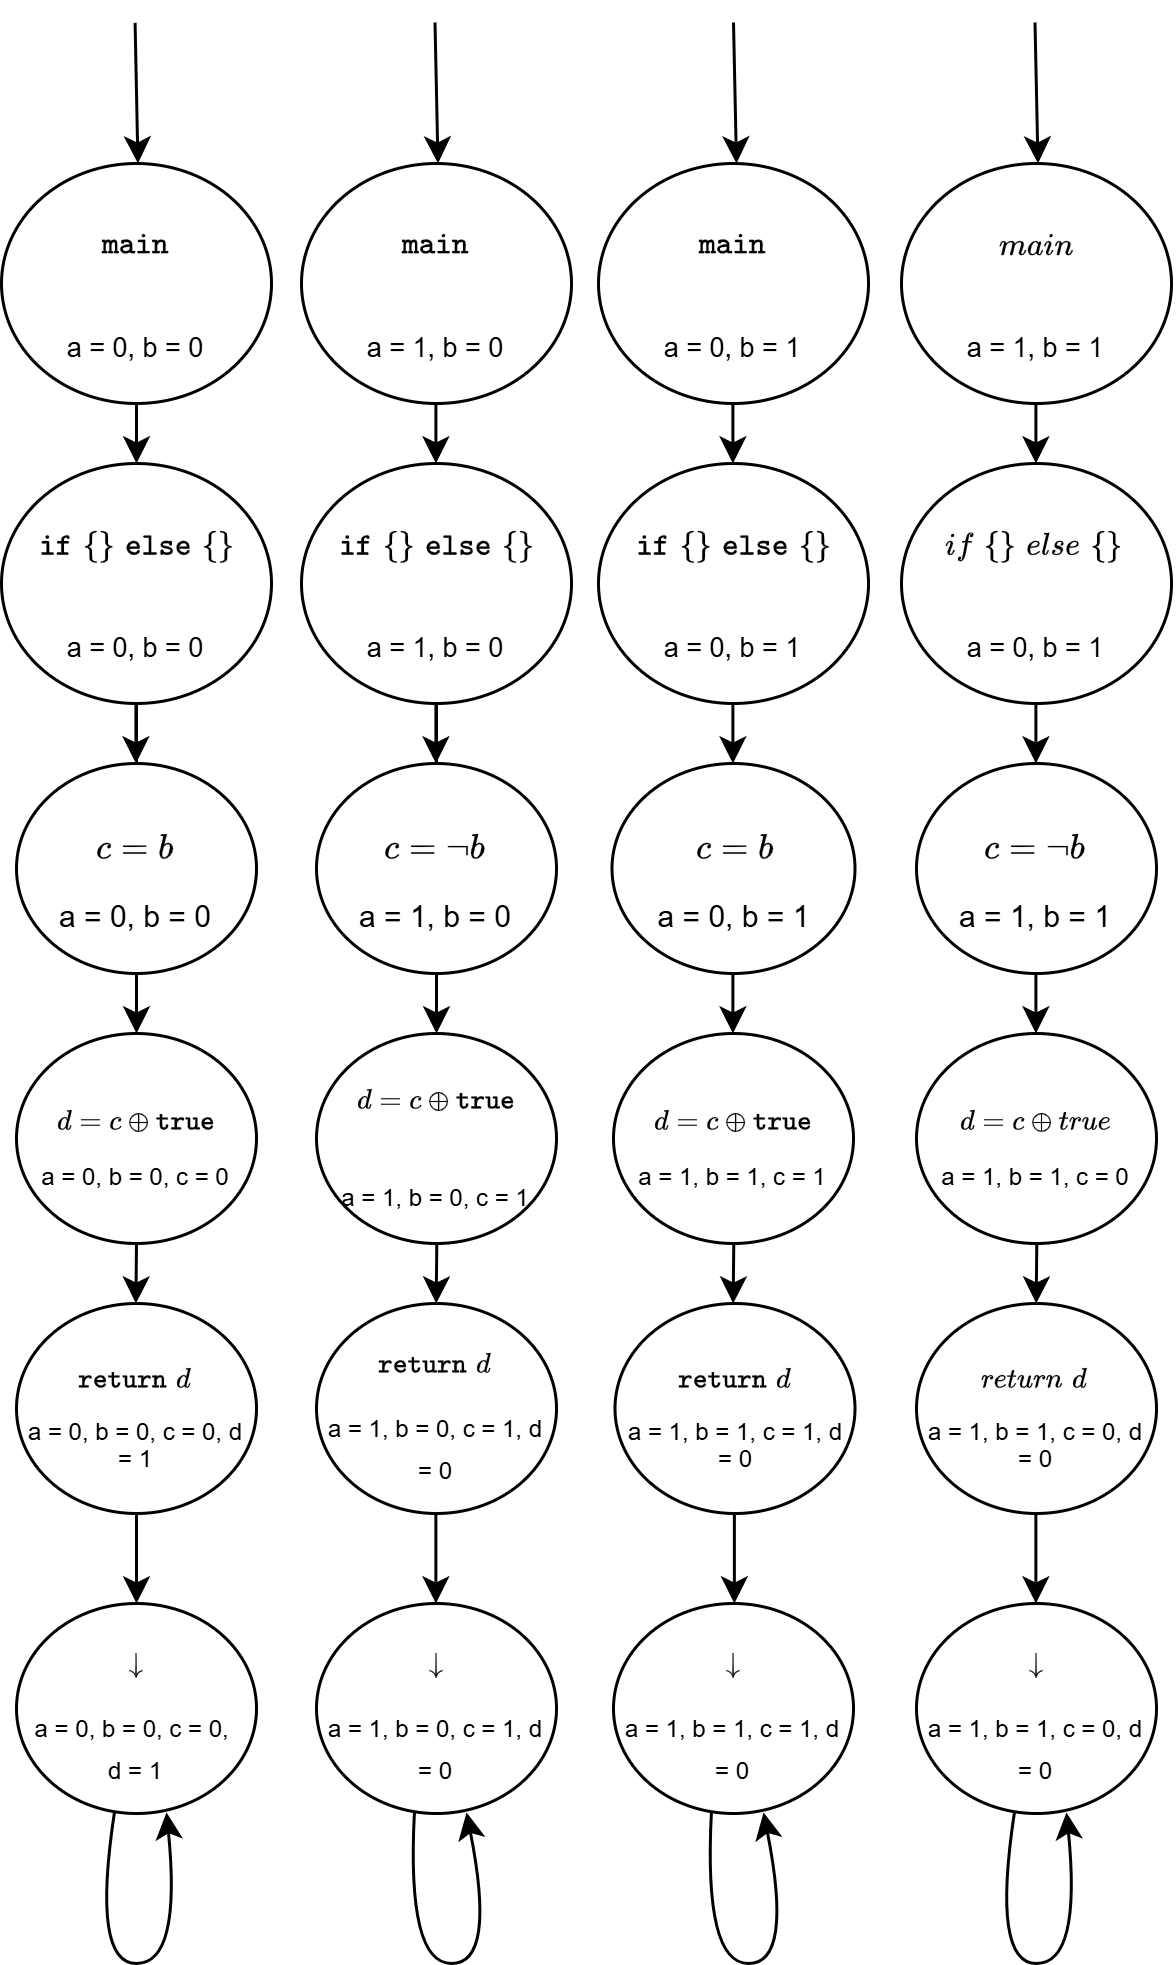
\includegraphics[scale = 0.20]{pictures/model-1.png}
    \end{center}
  \end{figure}

\clearpage

\section{Bonus Task: Project Management (50 P)}
\label{sec-bonus}

There is more to a successful project than just writing code. 
Usually, you also need to write proper documentation, distribute it, etc...

In this section, you will try some project management mechanisms for Haskell: 
In particular, you will provide documentation for your program, 
find the coverage of your test-suite and learn more about basic profiling with GHC.

\subsection{Command-Line Interface}

The program so far only has very rudimentary argument parsing, allowing a single or two filepath(s). 
However, anyone who did not write this program has no idea about how to invoke the Model Checker correctly, 
thus, we want to have a proper command-line interface.

\subsubsection*{Implementation Suggestions}

Common libraries for such tasks are \href{https://hackage.haskell.org/package/optparse-applicative}{\texttt{optparse-applicative}} 
and \href{https://hackage.haskell.org/package/cmdargs}{\texttt{cmdargs}} but it is also valid to not use any libraries at all 
and design your own solution.

\subsubsection*{Required Flags}

The program should be able to understand the following flags:

\begin{itemize}
\item On \code{-h}/\code{--help}, a help message should be displayed, explaining how the program can be invoked correctly.
\item On \code{--ts}, the input transition system should be parsed for correctness of the syntax of the input file, but no formula is verified on it.
\item On \code{--extensions}, a list of supported MiniCheck extensions is printed.
\item Other flags as you see appropriate. (optional, not graded)
\end{itemize}

\subsection{Documentation}

Document the most important types and functions of your project \href{https://haskell-haddock.readthedocs.io/en/latest/markup.html}{\texttt{haddock}}-conformly and provide the documentation via HTML.

Helpful commands:

\begin{itemize}
\item \code{cabal haddock} for building the documentation and inspecting it locally.
\item \code{cabal haddock --haddock-for-hackage} for building a \code{.tar.gz} containing the documentation.
\item \code{stack haddock --open}: builds documentation and opens it in the browser upon completion.
\end{itemize}

\subsection{Test Coverage}

Generate the test-coverage of your program's test-suite.
Discuss your findings and investigate any unexpected results.

Helpful commands:

\begin{itemize}
\item \code{cabal test --enable-coverage}
\item \code{stack test --coverage}
\end{itemize}

\subsection{Profiling}

Being able to profile your code is of great importance in real-world projects. Thus, we want you to experiment with some profiling in Haskell.

To do that, you might have to build your project in profiling mode:

\begin{itemize}
\item \code{cabal build --enable-profiling}
\item \code{stack build --profile}
\end{itemize}

Then you can pass RTS arguments to the GHC program to obtain run-time information, such as which function you spend the most amount of time in, etc...

Refer to the GHC documentation for the exact \href{https://downloads.haskell.org/ghc/latest/docs/html/users_guide/profiling.html#profiling-memory-usage}{\texttt{profiling flags}} to obtain relevant information.

Answer the following questions:

\begin{itemize}
\item What is the memory usage over time?
\item What is the peak memory usage?
\item Which function is the most time spent in?
\item Which type requires the most amount of memory?
\end{itemize}

\section{Submission Artefacts}
\label{sec:artefacts}

You should submit a zip-archive containing all project source files and a PDF with detailed project documentation in your group submission directory.

\subsection{Project Implementation}

The project should be written as a \code{cabal} or \code{stack} project consisting of multiple modules.

\subsection{Test Suite}

Unit tests and property tests need to be submitted as well, and it must be possible to run the whole test-suite with either \code{cabal test} or \code{stack test}.

\subsubsection*{Project Documentation}

The project documentation pdf should cover at least these topics and explain your choices.
\begin{itemize}
\item Which project build tool is used for the project? (\texttt{cabal} or \texttt{stack})
\item Which GHC version is used?
\item How can the program binary be built? How can it be run?
\item Which libraries are included as dependencies and which Haskell language extensions are enabled?
\item Which framework and libraries are used for writing tests?
\item Is the extension implemented?
\item How is the functionality partitioned into different modules?
\item How do you test your program? Which parts are the focus of your tests? Do there exist parts of the code that cannot be tested?
\item Are there known issues and limitations of your program?
\end{itemize}

%\vspace*{1cm}

\printbibliography




\end{document}


